\section{Network Function Chaining Infrastructure based on Virtualization Technologies} 
\subsection{Network Function Virtualization}
Traditionally carrier network has provided network functions (NF) like P-GW and S-GW on proprietary, dedicated hardware. However these hardware-based NFs have been being replaced by software, because of its high installation cost and relatively short lifetime. Furthermore flexible deployment of NF is required for the upcoming 5G wireless and Internet of Things (IoT). Since the software-based NFs are decoupled from the platform hardware, it is easy to newly deploy NF or withhold NF. 

Implementation of NF in software is realized by virtualization technology. This is called Network Function Virtualization (NFV). Virtualization technology is categorized into virtual machine (VM)-based and container-based technology. The former is full virtualization which creates virtual instances of hardware like CPU, RAM and network interface for every VM. Therefore a VM runs on a full copy on an operation system (OS) and virtual emulation of all needed hardware. A NF that runs as a VM is for these reasons resource consuming. The latter uses container-based technology represented by Docker\cite{Docker}. Container is a loosely isolated environment which runs on the kernel of host node. Isolation is done using five namespaces: process, network, mount, hostname, and shared memory. In contrast to VM, containers are light-weighted because each of them does not require virtualized resources.  

VM and container are used very commonly in NFV. A host can have multiple NFs (VMs or containers), and the traffic between NFs are exchangeable with software switches. Combined with software-defined network (SDN), traffic can be managed to go through specific NFs in other hosts. Either by chaining NFs in a single host or several hosts, a network service is created. In this paper, I propose a novel NF chaining mechanism inside of the kernel in a single host. 


\subsection{Advantage of VM-based/Container-based NFV}
The first advantage of using them is the portability of NFs. Any NF that is VM or Docker can operate on any other hosts that support these technologies. In case of VM, with XML file and image file and in case of Docker, with Dockerfile the same instance (VM or container) can be build. 

The second advantage is that the isolation is provided between instances (VMs or Containers). This enables the CPU, memory resources to be allocated to the instance as required. And the instance cannot take up more resources than allocated. 

\subsection{Disadvantage of VM-based/Docker-based NFV}
The main disadvantage is the packet forwarding: Each packet must be transmitted between NIC and instances (VM or Container) causing throughput bottleneck. I describe the detail of packet forwarding in VM-based and container-based technology, respectively in section 1.1.4 and 1.1.5. 

\subsection{Packet forwarding: VM-based NFV node}
In case of VM-based NFV, packet forwarding consists of three architectures, packet I/O, virtual network I/O and virtual switch. 
\begin{enumerate}
	\item Packet I/O: 
	 Packet I/O is the part where packets pass through between physical NIC and user space. The default of Linux is NAPI, but since the network stack of NAPI is considered redundant, there are acceleration technology like DPDK, XDP and Netmap to bypass network stack. DPDK provides libraries that enables user space process to directly access physical NIC's packet buffer. XDP and Netmap use memory mapping between NIC's packet buffer and user space's shared memory region, to give user space application direct access to packets. 
	\item Virtual network I/O: 
	Virtual network I/O mechanism is used for networking VMs and the underlying hypervisor. In KVM, each guest (VM) has virtio buffer where outgoing or incoming packets are stored. For the connection of virtio buffer and hypervisor, TAP interface is used. TAP interface is a software device with two endpoints: one is a NIC and the other one is file descriptor (fd). KVM process in the hypervisor send guest's tarffic to the fd endpoint of the TAP device. The traffic then arrives at the NIC endpoint which can be connected to other NIC or TAP interface using virtual switch. Finally the packets are written to the virtio buffer of the guest. The reversed path (traffic from guest to hypervisor) is followed similarly. Since writing to the virtio buffer is done by KVM process in user space, it involves system calls every time. To reduce the overhead by system call, vhost-net is available in KVM. With vhost-net enabled, kernel thread directly writes to the virtio buffer from TAP device, in stead of KVM process in the user space. 
	\item Virtual switch: 
	Virtual switch is used to forward traffic to the right port as mentioned above. Open Vswitch (OVS), which supports OpenFlow is representative among others. OVS uses flow table which has Match part and Action part. Match part is set of rules to filter packet and can distinguish not only 5 tuples, but also vlan tags or incoming port, etc. Action part can be drop, modify or transmit packet. When OVS works with virtual network I/O to realize NF chaining, the action should be transfer to specific L2 address port. 
\end{enumerate}

\subsection{Packet forwarding: Container-based NFV}
By default, docker uses local private network in the host. It creates virtual bridge and allocates subnet from one of the private address block. Each container gets allocated virtual ethernet device which is attached to the bridge. In this way, containers in the same subnet can communicate, if they are on the same host. 

Kubernetes project makes communication between containers on different hosts possible. In stead of allocating private IP address Kubernetes gives each pod (a group of containers) a global IP address, allowing NAT-less, flat address space. Either in the normal networking or Kubernetes's networking, network stack in the host is used to reach containers. 

\section{Overhead of NFCI based on Virtualization Technologies}
\subsection{Memory copy}
The recently dominating trend in NFV is to use VM or Docker container as Virtualized Network Function (VNF). However both of the technologies are not originally built in purpose of achieving high performance in heavy load network. 
Various kinds of efforts have been made to reduce the overhead of packet forwarding as mentioned in 1.1.3. For example, Netmap maps packet buffer into a memory region which user space process can directly access (zero-copy). But for the interaction with VM, software switch VALE which is supported on Netmap copies packets from the memory region to the guest's virtio buffer. Similary in case of DPDK + OVS, memory copy is needed to deliver traffic to VM. We believe that memory copy should be avoided to realize truly high performance NFV node.

Figure \ref{fig: kvm+ovs} shows the path of the traffic in a VM-based NFV node with KVM as virtual network I/O and OVS as virtual switch. With NAPI, traffic go through network stack (packet I/O) of the host, bridging by OVS, get input to virtio buffer of the guest and passed again through network stack in the guest. Even when bypassing packet I/O with DPDK or Netmap, traffic has to proceed unnecessary layers in order to be processed in a NF. 

Figure \ref{fig: docker} shows the path of the traffic when containers are used as NF and Docker Engine such as Kubernetes supports networking between them. Since container uses host's OS, traffic doesn't need to pass network stack once more inside the container, as in the case of VM-based node. But the path all the way up from NIC to 5th layer and forwarding in Docker Engine is yet not optimized for a truly high performance NFV node. 

\subsection{Resource Consumption}
In case of VM-based NFV, a NF consists of one or multiple VMs. To launch a VM, virtual instances such as CPU, memory and network I/O must be created. Since virtual instances are allocated for each of the VM, when managing several VMs it consumes lot of hardware resources. 

\begin{figure}[t]
	\begin{minipage}{0.5\hsize}
		\begin{center}
			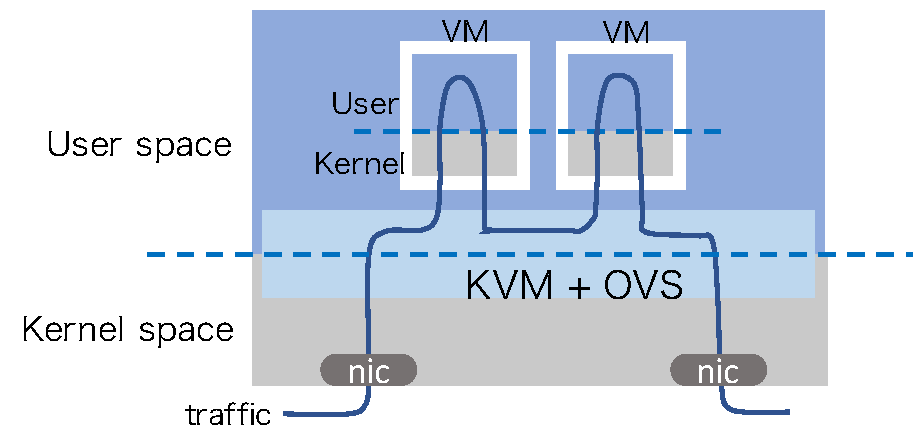
\includegraphics[width=85mm]{pics/KVM+OVS.pdf}
		\end{center}
		\caption{Traffic in VM-based NFV node}
		\label{fig: kvm+ovs}
	\end{minipage}	
	\begin{minipage}{0.5\hsize}
		\begin{center}
			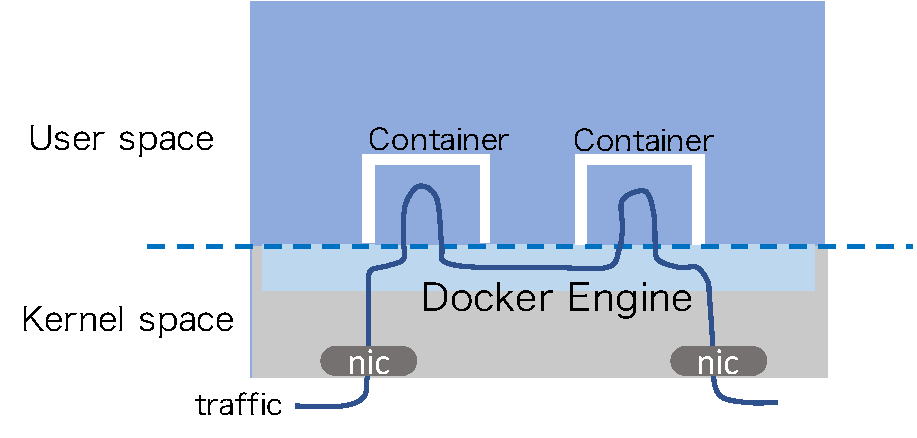
\includegraphics[width=85mm]{pics/Docker.pdf}
		\end{center}
		\caption{Traffic in Container-based NFV node}
		\label{fig: docker}
	\end{minipage}	
\end{figure}

\begin{figure*}
	\centering
	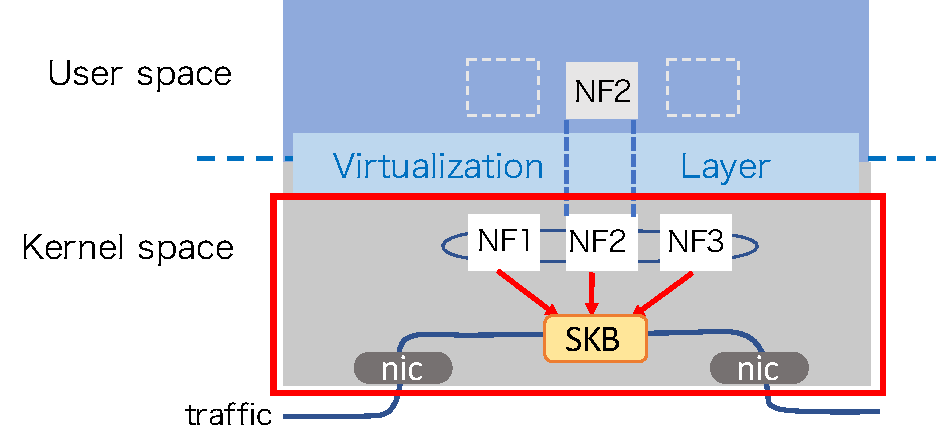
\includegraphics[width=95mm]{pics/path_kernel.pdf}
	\caption{Traffic in Kernel-based NFV node}
	\label{fig: path_kernel}
\end{figure*}

\section{Proposal: Lightweight NFC mechanism in Linux Kernel}
Because of the above two reasons, overhead in data path and resource consumption, we propose Kernel-based NFCI. Its aim is to realize lightweight NF chaining as much as possible in the kernel space on a single host. Simple and low load NFs should be executed in the kernel and NFs that require complicated tasks have to be put in the user space. The scope of this paper is the chaining mechanism for former NFs inside the kernel.

NF consists of one or more kernel modules. In order to integrate NF in network stack and manage traffic flow, we use Netfilter system in Linux. Netfilter is a set of hooks inside the kernel that allows kernel modules to register its functions. A registered function is called for every packet that traverses respective hook within the network stack. The NF chaining takes place in the first hook before the routing decision. 

As figure \ref{fig: path_kernel} shows, in our kernel-based NFCI node, NFs in kernel can directly access to the SKB because they are all in the same memory region. Therefore no need of memory copy. When a NF cannot be completely executed in the kernel, only the simple function is placed in the kernel and the rest must be put in user space by a virtualization technology. Because only complicated function is virtualized, overall resource consumption will be also decreased significantly. 

We think that certain amount of NFs consists of fairly simple functions and lots of them are feasible in the kernel. By providing a chaining mechanism for lightweight NFs in the kernel, overheads discussed so far will be largely eliminated. 

\subsection{Structure of the paper}
The structure of the paper is as follows. Related work is introduced in Chapter 2. In Chapter 3, the overall picture of the Kernel-based NFCI is described. Chapter 4 describes the architecture of the Kernel-based NFCI. In Chapter 5, the detail of the implementation is explained. An evaluation result is shown in Chapter 5. And finally, I conclude this study in Chapter 6. 











